\documentclass{article}
\usepackage{C:/Users/guitr/Documents/git_repositories/tpack/tpack}
% \usepackage{C:/Users/Admin-PC/Documents/git_repository/tpack/tpack}
% \usepackage{/home/tr0fin0/git_repositories/tpack/tpack}


\title{MI201 - Apprentissage Automatique}
\project{Résumé Théorique - kNN}
\author{Guilherme Nunes Trofino}
\authorRA{2022-2024}


\makeatletter
\begin{document}\selectlanguage{french}
\maketitle
\setlength{\parindent}{0pt}

\newpage\tableofcontents

\section{Introduction}
\subfile{C:/Users/guitr/Documents/git_repositories/classes_ensta/intro.tex}
% \subfile{C:/Users/Admin-PC/Documents/git_repository/classes_ensta/intro.tex}
% \subfile{/home/tr0fin0/git_repositories/classes_ensta/intro.tex}

\section{Apprentissage}
\subsection{Algorithme}
On considère que l'algorithme peut être définie par la définition suivante:
\begin{definition}
    Prédire la classe d'une nouvelle donnée en annotant les k plus proches voisins du donnée à classifier.
    \begin{figure}[H]
        \centering
        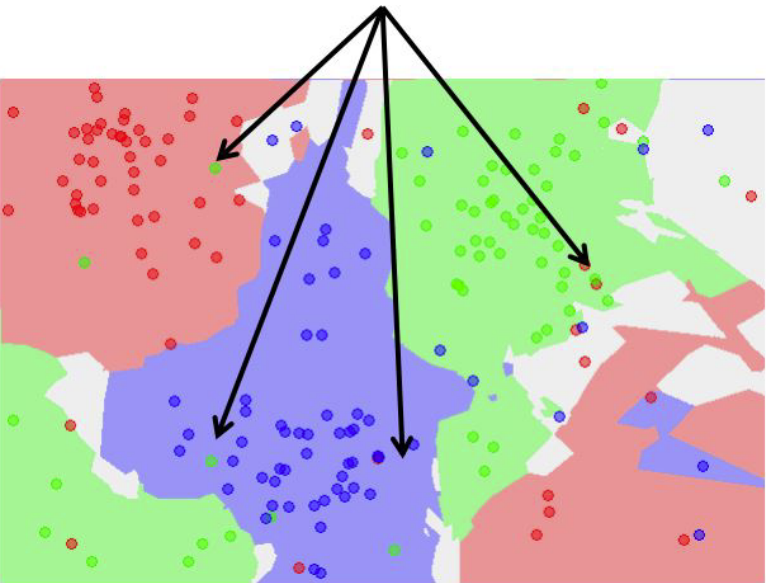
\includegraphics[height=60mm]{images/kNN_diagram.png}
        \caption{Representation kNN}
    \end{figure}
    La décision se fait pour le vote majoritaire, s'il n'y a pas de majorité la région reste blanche. 
\end{definition}
\begin{remark}
    On nomme kNN aussi comme kPPV, k Plus Proche Voisin en français.
\end{remark}
\begin{remark}
    kNN est très sensible aux données utilises, surtout aux bruits présentes. De cette façon-là il sera sensible à des pratiques comme la Validation Croisée.
\end{remark}
L'algorithme va définir une région pour chaque différent caractéristique de la base de données. En plus, chaque frontière sera une polynôme de plusieurs faces droites.\\

La choix de k déterminera la qualité de la prédiction. Si on augmente k la qualité de la prediction améliore et le sur-apprentissage diminue. Généralement on aura le comportement suivant:
\begin{table}[H]
    \centering\begin{tabular}{lll}
        k $\uparrow  $ & biais $\uparrow  $ & variance $\downarrow$\\
        k $\downarrow$ & biais $\downarrow$ & variance $\uparrow$\\
    \end{tabular}
    \caption{Comportement kNN}
\end{table}
\begin{remark}
    Quand le k devient trop grand, proche de la quantité de données, les prédictions de cet algorithme échouent car, ou lieu d'analyser les données, il va juste montre la caractéristique plus présent dans la base de données.
\end{remark}
On note qu'une variation très commun de cet algorithme est le 1NN:
\begin{definition}
    Prédire la classe d'une nouvelle donnée en annotant le plus proche voisin du donnée à classifier.
    \begin{figure}[H]
        \centering
        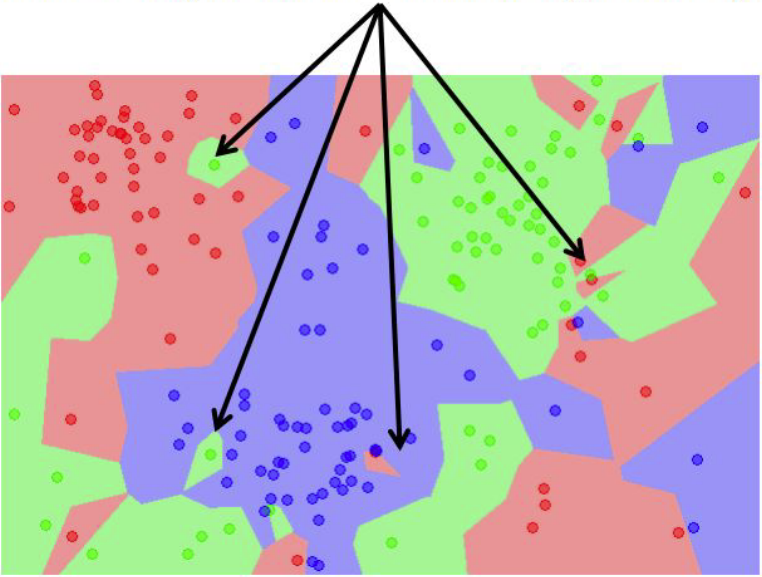
\includegraphics[height=60mm]{images/1NN_diagram.png}
        \caption{Representation 1NN}
    \end{figure}
\end{definition}
\begin{phrase}
    Tous les sensibilités de kNN seront encore plus grand dans 1NN.
\end{phrase}

\subsubsection{Avantages}
Dans ce cas, cet algorithme	est très simple à implementer et facile à comprendre.
\subsubsection{Incovenients}
Dans ce cas, cet algorithme est très sensible aux données et le coût de prédiction croît en $O(nd)$.  
\subsubsection{Applications}
Cet algorithme est souvent utilisé pour l'interpolation des données


% \subsection{Initialization}
% \subsection{Visualization}
% \subsection{Training}



% \section{Prédiction}
% \subsection{Analyses}
\end{document}